\documentclass[10pt]{article}
\usepackage[top=0.85in,left=2.5in,footskip=0.75in]{geometry}
% amsmath and amssymb packages, useful for mathematical formulas and symbols
\usepackage{amsmath,amssymb}

% Use adjustwidth environment to exceed column width (see example table in text)
\usepackage{changepage}

% Use Unicode characters when possible
\usepackage[utf8x]{inputenc}

% textcomp package and marvosym package for additional characters
\usepackage{textcomp,marvosym}

% cite package, to clean up citations in the main text. Do not remove.
\usepackage{cite}

% Use nameref to cite supporting information files (see Supporting Information section for more info)
\usepackage{nameref,hyperref}

% line numbers
\usepackage[right]{lineno}

% ligatures disabled
\usepackage{microtype}
\DisableLigatures[f]{encoding = *, family = * }

% color can be used to apply background shading to table cells only
\usepackage[table]{xcolor}

% array package and thick rules for tables
\usepackage{array}

%% The graphicx package provides the includegraphics command.
\usepackage{graphicx}
%% The amssymb package provides various useful mathematical symbols
\usepackage{amssymb}
%% The amsthm package provides extended theorem environments
%% \usepackage{amsthm}
%% I cannot believe how little functionality is included natively in \LaTeX
\usepackage{rotating}
%% Some packages for less awful tables
\usepackage{booktabs}
\usepackage{tabularx}
\usepackage{array}
%% It's designed for scientific reports and yet crashes if you use SI!
\usepackage{siunitx}
%% It doesn't support text subscripts! It doesn't even document well that it doesn't support text subscripts!
\usepackage{tikz}
%% It doesn't support degree signs
\usepackage{textcomp}
\usepackage{pdflscape}
\usepackage{colortbl} 
\usepackage{xcolor} 
\usepackage{xfrac}
\usepackage[title]{appendix}
\usepackage{hyperref}
\hypersetup{final}
\usepackage{threeparttable}
\usepackage{scalefnt}
\usepackage{amssymb}
\usepackage{cleveref}
\usepackage{float}
\usepackage{amsmath}
\usepackage{setspace}

%% Keeps tables looking tolerable.
\newcolumntype{K}{>{\centering\arraybackslash}m{4cm}}
\newcolumntype{L}{>{\centering\arraybackslash}m{2.7cm}}
\newcolumntype{M}{>{\centering\arraybackslash}m{3cm}}
\newcolumntype{N}{>{\centering\arraybackslash}m{1.2cm}}
\newcolumntype{O}{>{\centering\arraybackslash}m{0.5cm}}
\newcolumntype{P}{>{\centering\arraybackslash}m{2.2cm}}

%% That perfect ggplot grey for consistency
\definecolor{gggrey}{RGB}{230,230,230}

%% Seeing as this is going to be submitted electronically, I think we can sacrifice page count at the altar of readability. 
\setlength{\parskip}{1em}

\usepackage{lineno}

\newcolumntype{+}{!{\vrule width 2pt}}

% create \thickcline for thick horizontal lines of variable length
\newlength\savedwidth
\newcommand\thickcline[1]{%
  \noalign{\global\savedwidth\arrayrulewidth\global\arrayrulewidth 2pt}%
  \cline{#1}%
  \noalign{\vskip\arrayrulewidth}%
  \noalign{\global\arrayrulewidth\savedwidth}%
}

% \thickhline command for thick horizontal lines that span the table
\newcommand\thickhline{\noalign{\global\savedwidth\arrayrulewidth\global\arrayrulewidth 2pt}%
\hline
\noalign{\global\arrayrulewidth\savedwidth}}

% Apparently aligning a title to the left is too complex for \LaTeX
\makeatletter
\renewcommand{\maketitle}{\bgroup\setlength{\parindent}{0pt}
\begin{flushleft}
  \textbf{\@title}

  \@author
\end{flushleft}\egroup
}
\makeatother

% Text layout
\raggedright
\setlength{\parindent}{0.5cm}
\textwidth 14cm
\textheight 8.75in

% Bold the 'Figure #' in the caption and separate it from the title/caption with a period
% Captions will be left justified
\usepackage[aboveskip=1pt,labelfont=bf,labelsep=period,justification=raggedright,singlelinecheck=off]{caption}
\renewcommand{\figurename}{Fig}

% Use the PLoS provided BiBTeX style
\bibliographystyle{plos2015}

% Remove brackets from numbering in List of References
\makeatletter
\renewcommand{\@biblabel}[1]{\quad#1.}
\makeatother

% Header and Footer with logo
\usepackage{lastpage,fancyhdr,graphicx}
\usepackage{epstopdf}
%\pagestyle{myheadings}
\pagestyle{fancy}
\fancyhf{}
%\setlength{\headheight}{27.023pt}
%\lhead{\includegraphics[width=2.0in]{PLOS-submission.eps}}
\rfoot{\thepage/\pageref{LastPage}}
\renewcommand{\headrulewidth}{0pt}
\renewcommand{\footrule}{\hrule height 2pt \vspace{2mm}}
\fancyheadoffset[L]{2.25in}
\fancyfootoffset[L]{2.25in}
\lfoot{\today}

%% Include all macros below

\newcommand{\lorem}{{\bf LOREM}}
\newcommand{\ipsum}{{\bf IPSUM}}

%% END MACROS SECTION
\title{\Large{Are regulatory limits on pollutants sufficient to protect from emergent mixture effects?}}
\author{Samuel A. Welch\textsuperscript{1}}

\begin{document}

\begin{flushleft}
\maketitle
\bigskip
\textbf{1.} Department of Life Sciences, Silwood Park, Imperial College London, United Kingdom
\bigskip
\end{flushleft}
\vspace{1.3cm}

\begin{center}

\includegraphics[scale = 0.4]{docs/badnews8ways.png}

\vspace{1.3cm}

A thesis submitted in partial fulfilment of the requirements for the degree of Master of Science at Imperial College London\\
\smallskip
Formatted in the journal style of \textit{PLOS}\\
\smallskip
Submitted for the MSc in Ecological Applications
\end{center}

% Please keep the abstract below 300 words
\section*{Abstract}
Longstanding ecotoxicological convention is that interaction between complex mixtures of three or more chemical stressors are negligible compared to two-way interactions. Recent studies on \textit{E. coli} exposed to complex mixtures of antibiotics, however, have suggested this is not the case. This study set out to determine if this new evidence were applicable to wild soil bacteria and communities exposed to 255 1-8-way combinations of eight heavy metals, pesticides and antibacterials.

Our findings suggest that experimental results from exposures of lab species may not be applicable to wild species. Of the seven isolates and one soil community studied, although many non-significant non-additive effects were detected, only \textit{E. coli} OP50, a lab strain, showed significantly non-additive effects (n = 777, $p < 0.05$), and almost no 'emergent effects', mixture effects not predictable from their components at a level of complexity one smaller, were detected. A comparison of nested linear models suggested that across the studied isolates, two-way interactions were the most significant in determining mixture effect on growth (F = 6.41, F-critical = 1.04, $p < 0.05$).  

It thus appears that present regulatory limits on chemical stressor concentrations in the environment do protect bacteria from mixture effects, over short exposures. More research is needed to determine how applicable these results are to real-world exposures. 

\newpage

\begin{spacing}{0.05}
\tableofcontents
\end{spacing}
\vspace{0.5cm}
\textit{This table of contents is included for ease of navigation.}

\newpage

\section*{Declaration} 

Drs Emma Ransome (ER), Tom Bell (TB) and Shorok Mombrikotb (SM) assisted in the design of experimental protocols and parts of the design of the statistical analysis. SM also assisted with the design of the worklists for the Hamilton STARlet, and provided Nash's Field soil isolates for experimental use.

Nilita Mukjang assisted with the sampling and preparation of soil microbial communities.

I conducted all aspects of the data collection, cleaning and analysis, including all code used in cleaning and analysis. As part of this process I made use of a number of R packages, which are cited in Methods (\cref{S:3}).

\linenumbers

%% main text
\section{Introduction}
\label{S:1}

Any organism today must contend with not only a broad range of ecological and biogeographic stressors, but also the presence of more than 100 million known chemicals \cite{CAS2015}. Though many of these chemicals have always been naturally present in the world as components of the crust, secreted biocides or waste products, complex mixtures of chemical stressors are now a common feature in terrestrial and aquatic ecosystems. \cite{EuropeanCommission2012a}. 

Though mixture toxicity has long attracted much academic attention \cite{Bliss1939}, criticisms remain of a lack of consensus on experimental design, use of statistics, and even inconsistent interaction definitions \cite{Jackson2016,Piggott2015,Schafer2018}. Ecotoxicology still bears the legacy of its largely regulatory past: a preoccupation with declaring any given chemical safe or not, using a limited panel of model species \cite{OECD2014SectionSystems}. Equally, existing mixture toxicity regulations in the EU are limited and distinctly human-focused \cite{EuropeanCommission2012a}, and do not represent the latest in scientific knowledge.

A longstanding criticism of ecotoxicology remains the difficulty of integrating ecotoxicological results into a broader understanding of how ecosystems respond to stress across their component species. \cite{Chapman2002a,Gessner2016}. Ecosystems are without exception supported by a broad trophic foundation of microbes that provide vital services as decomposers, chemical engineers, and pathogens \cite{Nannipieri2003a,VanderHeijden2008a}, but in regulatory and scientific settings a chemical's toxicity to bacteria is typically tested using the luminescent bacteria toxicity assay (LBTA) \cite{OECD2014SectionSystems}, a 30-minute exposure to \textit{Aliivibrio fischerii}, a bioluminescent marine decomposer. The LBTA is the industry standard due to its simplicity and ease of use, but it suffers from a number of well-documented limitations \cite{Ma2014} in addition to the difficult of generalising from one species to an entire ecosystem.

Constrained by practical limitations, ecotoxicology experiments have always tended towards simplicity. Studies have traditionally consider the effects of a single stressor on a single species, and where stressor interaction has been examined, it has been largely limited to binary mixtures of stressors \cite{Peterson2017}. In brief summary, two chemicals or environmental factors, that are known to have a positive or negative effect on some aspect of a species' fitness, are mixed at various concentrations. By comparing their observed effect to a null hypothesis prediction of their effect calculated by adding (or in some cases multiplying \cite{Schafer2018}) individual effects, it is possible to determine the nature of the interaction between stressors in a mixture (\cref{tab:simple_interactions}). A result not significantly different from the null hypothesis is considered additive, a result significantly larger is synergistic, and a result significantly smaller is antagonistic. 

\begin{table}[ht]
\centering
\begin{tabular}{l l}
\toprule 
\textbf{Name} & \textbf{Observed Effect vs Predicted Effect} \\
\midrule
\rowcolor{gggrey}   Additivism      &   \textit{Observed effect $\approx$ sum of individual effects} \\
                    Synergy         &   \textit{Observed effect $>$ sum of individual effects} \\
\rowcolor{gggrey}   Antagonism      &   \textit{Observed effect $<$ sum of individual effects} \\
\bottomrule
\end{tabular}
\caption{Conventional definitions of interactions between stressors, based on Bliss \cite{Bliss1939}}
\label{tab:simple_interactions}
\end{table}

Though easy to understand and employ, this model is not without its issues. Confusion over definitions abound. For instance, the term 'stressor' is often used as a synonym for 'pollutant', 'toxicant', or 'pressure' -- a substance or treatment that produces a negative fitness effect in the species of interest \cite{Piggott2015}. However, not only does this fail to account for the well-known adage that 'the dose makes the poison'\cite{OGParacelsus} –- as true for a rise in temperature or in nutrient availability as it is for toxic pollutants -- but also that \textit{the species makes the poison}. Many organisms, particularly bacteria, are are able to tolerate or even thrive on substances that are harmful to other species \cite{Malik2004,Gadd2009}. 

Due to the geometrically-increasing complexity of adding additional stressors to interaction experiments, the number of studies that have experimentally examined the interactions of mixtures of three or more chemicals –- 'higher order interactions' –- has been limited \cite{Beppler2016}. This has been justified by a long-held assumption that higher-order interactions are negligible compared to lower-order interactions \cite{Tekin2017a}, but recent studies examining complex mixtures of antibiotics have shown emergent higher-order effects,  three-way interactions not predictable from component two-way effects, meaning that the existing body of binary-interaction based literature may not be scalable over more complex mixtures to understand the effects on ecosystems \cite{Tekin2016, Zimmer2016, Tekin2017}. Within ecology, research on complex combinations of stressors -– including chemicals –- is more common, and suffers from similar uncertainty and confusion in defining synergy and antagonism \cite{Cote2016}.  Beppler \textit{et al.} also highlight the study of emergent interactions between higher-order mixtures of predators -– Multiple Predator Effects (MPEs) –- that has received some attention. One recent review of the literature \cite{Griffin2013EffectsMeta-analysis} found overall that species-rich mixtures of predators were more effective at suppressing prey than poorer mixtures, although a considerable number of component studies found no significant relationship. 

Parallels can also be drawn with research on inter-species interactions in the vein of food webs, the presence of a species having a positive or negative effect on the fitness of other species in a similar manner to a chemical stressor. Considerable research has explored interaction across food webs and trophic levels, and the  cascading shifts in biotic interactions caused by abiotic environmental change \cite{Hooper2005,Parmesan2006,Chesson2000}. Research has shown that chemical stressors such as pesticides can cause large scale changes over short timescales to ecosystems, mediated through complex webs of interactions \cite{Thompson2016}. The effect of species interaction on evolutionary responses has also been examined species interaction \cite{Lawrence2012}, showing that in bacteria these interactions can over time cause considerable shifts in both communities and the phenotypes and genotypes of component species.

In the Anthropocene, an era where pollution is a greater pressure on ecosystems than ever before, it is vital that we improve our understanding of how a diverse range of wild bacteria respond to different stressors. Greater understanding of these stressors and interactions will enable more targeted and cost-efficient legislation and interventions -– for instance, one stressor has a disproportionate effect on overall response and thus should produce the greatest positive effect when removed. 

This study thus aims to address this knowledge gap by examining the effects of complex mixtures of common pollutants on a diverse panel of soil bacteria. It is hypothesised that more complex mixtures of chemicals will produce emergent effects not predictable from studying the chemicals in isolation, and that single stressor responses and interaction responses will vary across the bacterial panel.

\section{Methods}
\label{S:2}
\subsection{Isolate Selection}
\label{S:2:1}

Eight bacterial isolates were selected, sourced principally from the Nash's Field experimental site at Silwood Park, United Kingdom. Since 1991, plots within Nash's Field have been treated three times yearly with metaldehyde at 960 g/ha as part of herbivore exclusion experiments \cite{Allan2011ContrastingExperiment} (\cref{A:2}). The bacteria used in this study were isolated and sequenced form plots with different exposure histories (\cref{tab:isolates}) in 2016 for an earlier study \cite{Mombrikotb2016}. 

\begin{table}[ht]
\begin{small}
\centering
\begin{tabular}{c p{3.1cm} l p{5.2cm}}
\toprule 
\textbf{{Strain}} & \textbf{{Species}} & \textbf{{History}} & \textbf{{Notes}} \\
\midrule
\rowcolor{gggrey}{LUF4\_5} & \textit{Luteibacter rhizovicinus} & Control & First isolated from the rhizosphere \cite{Johansen2005LuteibacterL.}. \\
{KUB5\_13} & \textit{Variovorax paradoxus} & Control & Strains capable of metabolising a wide range of pollutants \cite{Satola2013MetabolicParadoxus}. \\
\rowcolor{gggrey}{NUF1\_3} & \textit{Variovorax paradoxus} & Metaldehyde & \\
{KUE4\_4} & \textit{Bacillus simplex} & Control & Strains capable of biosorption of heavy metals and radionuclides \cite{Valentine1996BiosorptionZone}. \\
\rowcolor{gggrey}{NUE1\_1} & \textit{Bacillus simplex} & Metaldehyde & \\
{KUE4\_10} & \textit{Stenotrophomonas \newline acidaminiphila} & Control & First isolated from a waste-acid-treating anaerobic bioreactor \cite{Assih2002}. \\
\rowcolor{gggrey}{OP50} & \textit{Escherichia coli} & Control & \textit{Caenorhabditis elegans} feeder\cite{Stiernagle2006}, included as a model species. \\
{KUA5 Sample} & Soil Community & Control & \\
\bottomrule
\end{tabular}
\caption{Bacterial species, strains, and sources.}
\label{tab:isolates}
\end{small}
\end{table}

Isolates were stored on CryoBeads in a standard \textit{Brucella} broth with glycerol solution (Hardy Diagnostics, CB12) at -80\textdegree C until needed for experiments, when they were cultured overnight on a rotary shaker (140 RPM) in a standard R2A broth at room temperature (25.9\textdegree C –- 26.6\textdegree C) prior to experiments. Soil communities were frozen in a 60\% glycerol solution immediately after extraction and defrosted on an individually for overnight culturing. 

\subsection{Stressor Selection}
\label{S:2:2}

Chemical stressors were selected from a range of categories (\cref{tab:stressors}) in order to assemble a panel that had some common mechanisms of action, and that have the potential to occur in mixtures in ecosystems.

Nickel (\textsubscript{28}Ni) and Copper (\textsubscript{29}Cu) are heavy metals, common pollutants with a wide range of industrial applications. Copper is an essential respiratory nutrient across all kingdoms of life \cite{Babcock1992}, while nickel is a cofactor in many bacterial and fungal enzymes \cite{Zamble2015}. Bacterial resistance to these stressors is thus often nuanced, with a need to balance availability in the cell as nutrients with their potential for damage.  Copper is a prolific generator of Reactive Oxygen Species (ROS) \cite{Bal2002}, and damages vital biosynthesis enzymes \cite{Macomber2009}, while nickel is a weak ROS generator, and can dangerously unbalance iron and zinc homeostasis in the cell \cite{Samland2006}. Copper and nickel are resisted through similar pathways \cite{Mykytczuk2011CytoplasmicFerrooxidans}, including active efflux and membrane modification. Copper is also resisted through chelation and rapid repair of damaged enzymes \cite{Macomber2009}, while nickel can be sequestered in vacuoles within the cell \cite{Nishimura1998}.

Chloramphenicol and ampicillin are broad spectrum antibacterial agents, effective against many gram-positive and -negative bacteria, and used in decreasing quantities in healthcare applications due to their severe side effects and growing resistance. Nevertheless, as well-studied environmental pollutants they are ideal candidates for exposures. First isolated from \textit{Streptomyces venezuelae}, a soil-dwelling bacterium, chloramphenicol is a broad-spectrum antibiotic, to which resistance in the wild and areas under antibiotic pollution is particularly common \cite{Allen2010}. Ampicillin, a widespread antibiotic from the penicillin family, is also widely resisted \cite{Ruiz1999MechanismsFish}. Chloramphenicol acts bacteriostatically by inhibiting protein synthesis in the 50S ribosomal subunit, while ampicillin inhibits cell wall synthesis. Drug interaction studies have shown that chloramphenicol is negatively antagonistic towards ampicillin, due to their competing modes of action \cite{vanBambeke2017MechanismsAction}. It has been suggested that many of the genes that provide resistance to common antibiotics, including chloramphenicol, also provide tolerance to environmental stress \cite{Groh2007}. Research has also shown that exposure to ROS from heavy metals, including copper, can co-select for chloramphenicol resistance \cite{Harrison2009}.

Atrazine, a triazine herbicide, has been banned in the EU since 2004 \cite{EU2004}, but has remained the most commonly used herbicide in the US, and acts on plants by disrupting photosynthesis \cite{Shimabukuro1969}. Atrazine has been shown to be both a food source \cite{Wackett2002} and ROS stressor \cite{Zhang2012} to various species of bacteria. Metaldehyde, a common water pollutant and mollusicide, is rapidly converted within the body of its target species into aldehyde, which damages mucus producing cells, causing excessive mucus production, dehydration, and eventual death \cite{Triebskorn1998}. However, knowledge of its effects on bacteria are limited -- only one study has examined interactions between bacteria and metaldehyde \cite{Thomas2017}, showing only that \textit{Variovorax} and \textit{Aceinetobacter} strains can be isolated from metaldehyde-treated soil, and can degrade the molluscicide.

Tebuconazole is a triazole fungicide that acts against a broad range of pathogens by inhibiting fungi-specific membrane synthesis pathways. Tebuconazole is known to be toxic to a range of non-target species \cite{Sehnem2010}, but information on effects on bacteria is limited to the knowledge that some bacteria -- though none of the species used in this study -- are capable of degrading tebuconazole \cite{Sehnem2010}. Azoxystrobin is a systemic fungicide in heavy use due to its broad-spectrum inhibition of respiration across major groups of fungal pathogens. Azoxystrobin has been shown to inhibit bacterial growth in mixed fungal-bacteria communities \cite{Bacmaga2015MicrobialAzoxystrobin}, although the same study showed \textit{Bacillus} species were capable of growth in highly contaminated soil.

Limited data are available on the prevalence and composition of chemical mixtures in waters in the UK. However, hospital effluent is known to represent an important source of not only anti-bacterial pollution \cite{Sacher2001} but also heavy metals \cite{Verlicchi2010}. Agriculture is also a potential source of complex chemical mixtures, through the simultaneous use of fungicides, herbicides, insecticides, veterinary antibiotics \cite{Stuart2012}, while heavy metals frequently enter the environment through industrial wastewater, mine run-off, and landfill leachate \cite{Facchinelli2001}. Where pollution from these sources mix, such as at the interface between different land uses, or in the body of a river that runs through such areas, chemical mixtures are likely to be common.

%% LaTeX was sent to punish us for our sins.
%% I've got no idea what they were, but they must have been pretty bad for us to end up with LaTeX.

\begin{landscape}
\begin{table}[h]
\begin{threeparttable}
\small
\setlength{\tabcolsep}{4pt}
\setlength{\extrarowheight}{3pt}
\begin{tabular}{l M l K K K c}
\toprule
\textbf{Stressor} & \textbf{Functional Group} & \textbf{Limit (\SI{}{\ug}/l}) & \textbf{Form/Product Code} & \textbf{Bacterial mechanisms of action} & \textbf{Bacterial mechanisms of resistance} & \textbf{Sources} \\
\midrule
\rowcolor{gggrey}\textbf{Copper} & Heavy Metal & 2000\tnote{t} & Cu(II)Cl\textsubscript{2}, dihydrate (99\%), Alfa Aesar 12458 & Essential nutrient, ROS, enzymes & Efflux, chelation, rapid repair, membrane transition & \cite{Nayar2004EnvironmentalMesocosms,Valko2005,Dupont2011,ECHA2018Cu} \\
\textbf{Nickel} & Heavy Metal & 20\tnote{t} & Ni(II)Cl\textsubscript{2}, anhydrous (98\%), Alfa Aesar B22085 & Enzymes, Fe/Zn homeostasis, weak ROS, nutrient & Sequestration, efflux, membrane transition & \cite{Nayar2004EnvironmentalMesocosms,Macomber2011,Nishimura1998,Zamble2015} \\
\rowcolor{gggrey}\textbf{Chloramphenicol} & Antibacterial & 0.05\tnote{n} & Powder $\geqslant$98\%, Sigma Aldrich C0378 & Cell wall synthesis & Membrane transition, mutant ribosomes, anti-AB enzymes & \cite{Shaw1979,Rebstock1949,Toku-E2018Ch,Ruiz1999MechanismsFish} \\
\textbf{Ampicillin} & Antibacterial & 0.12\tnote{n} & Ampicillin sodium salt, Sigma Aldrich A9518 & Protein synthesis, 50S ribosome subunit & $\beta$-lactamase enzymes, efflux & \cite{Ruiz1999MechanismsFish,Costanzo2005} \\
\rowcolor{gggrey}\textbf{Atrazine} & Pesticide (Herbicide) & 0.25\tnote{t} & Power, analytical, Sigma Aldrich 45330 & ROS, bacterial enzymatic nutrient & Biodegradation & \cite{Shimabukuro1969,Delorenzo2001,Zhang2012} \\
\textbf{Metaldehyde} & Pesticide \break (Insecticide) & 0.5\tnote{t} & Powder, analytical, Sigma Aldrich 63990 & Toxicity unknown, possible nutrient & Biodegradation & \cite{Kay2014,Castle2017,Thomas2017} \\
\rowcolor{gggrey}\textbf{Tebuconazole} & Antibacterial & 1\tnote{r} & Ampicillin sodium salt, Sigma Aldrich 32013 & Unknown & Biodegradation & \cite{Sehnem2010,Artigas2014ComparativeEcosystems} \\
\textbf{Azoxystrobin} & Antibacterial & 3\tnote{r} & Powder, Analytical, Sigma Aldrich 31697 & Unknown & Biodegradation & \cite{Battaglin2011Occurrence20052006,Rodrigues2013,Loos2010,Bacmaga2015MicrobialAzoxystrobin} \\
\bottomrule
\end{tabular}
\caption{Summary of stressors including type, target concentration, product information and bacterial interactions.}
\label{tab:stressors}
\begin{tablenotes}
\item [t] UK drinking water regulatory limit, Water Framework Directive
\item [n] No legal limit, typical environmental concentrations used.
\item [r] Regulatory Acceptable Concentrations, Water Framework Directive 
\end{tablenotes}
\end{threeparttable}
\end{table}
\end{landscape}

%% There! A table that look five times as long to produce as in Word, and is twice as ugly.

\subsection{Rangefinding and Concentration Calculations}
\label{S:2:3}

Initial dose-response exposures were conducted at concentrations above and below regulatory limits to determine individual stressors' effects on isolates. Eight 96-well microtiter plates were prepared, with  \SI{10}{\ul} of 1-in-100 diluted overnight culture, \SI{80}{\ul} of R2A broth, and \SI{10}{\ul} of stressor stock at either 0.1, 1, 10 or 100 times the target final experimental concentration added to each well. Each well of stressor concentration and isolate was replicated three times. Well OD was read using the cell count protocol below \ref{S:2:4}.

Final experimental concentrations were chosen based on regulatory limits where available, and realistic environmental concentrations where no regulatory limits exist (Limits column, \cref{tab:stressors}). Calculations are available in Appendix \ref{A:1}.

\subsection{Metrics of Growth}
\label{S:2:4}

Microcosm optical density (OD) at 590 nm was used as a metric of cell count over time. Immediately after isolates were exposed to stressors, plates were placed in an automatically-fed BioTek Synergy 2 microplate reader for 48 hours, agitating the wells for 5 seconds then reading absorbance every four hours.  At the conclusion of OD readings, wells were checked for contamination by plating the contents of the control plate at $10^{-3}$ and $10^{-4}$ dilutions onto a R2A agar plate and culturing at room temperature for 24 hours.

Flow cytometric cell counts, read in an Accuri C6 Flow Cytometer, were plotted against optical density using a linear model in an attempt to transform OD reading into absolute cell counts. However, no significant relationship was found between the two measurements, as at the time of measurement, cell counts were insignificantly high to be detected as changes in optical density (Appendix \ref{A:1}). 

Optical density was modelled against time in hours using a logistic curve, selected as a well-documented and fitting model \cite{Zwietering1990}.  from the package \textit{growthcurver} \cite{Sprouffske2016Package} for the R programming language \cite{RCoreTeam2018}.

\begin{equation}
Nl_t=\frac{K}{1 + (\frac{K - N_0}{N_0}) e^{-rt}}
\label{E:log_curve}
\end{equation}

Growth data and logistic curve were plotted by well, allowing for visual inspection and the exclusion of models from wells where no growth had occurred as a result of factors other than stressor treatment. A null additive model was assumed for all comparisons, consistent with the use of bacterial growth as a metric of response \cite{Piggott2015}. 

A typical bacterial growth curve \cite{Monod1949} offers a number of potential parameters for the quantification of bacterial growth, summarised in \cref{tab:metrics} below. Of the metrics available, the unitless measure of empirical area under the curve ($auc\_e$ in \textit{growthcurver)} was selected, as its use did not involve the same loss of exponential phase growth data as in measurement of lag time, carrying capacity, or level of growth at a specific time point. Growth level, which involves the fitting of a Zwietering logistic growth curve to measured growth and the extraction of parameters from the curve, was not considered as a metric due to a lack of awareness during the data analysis phase \cite{Cuevas2017}. Growth score, a refined form of growth level, was rejected for the same reason \cite{Cuevas2018}.

\begin{table}[ht]
\centering
\scriptsize
\renewcommand{\arraystretch}{1.8}
\begin{tabular}{P M L L N}
\toprule 
\textbf{Metric} & \textbf{Description} & \textbf{Advantages} & \textbf{Disadvantages} & \textbf{Example/ Citation} \\
\midrule
\rowcolor{gggrey}{Lag time} & Time before bacterial growth phase & Provides high level of resolution over initial growth phase & Ignores variation in other phases & \cite{Monod1949} \\
{Area under curve (auc)} & Area under logistic or empirical growth curve & Accounts for effects at all phases of growth & Loss of growth resolution & \cite{Firsov2001} \\
\rowcolor{gggrey}{Carrying capacity $k$} & Maximum growth (stationary phase) & Better accounts for variable growth speed between species & Ignores variation in other phases & \cite{Chapman2018} \\
{Growth\textsubscript{t}} & Growth as measured at a consistent timepoint & Easy to measure & Considerable loss of resolution & \cite{Hall2014} \\
\rowcolor{gggrey}{Growth Level (GL)} & Least-squares fitting of Zwietering logistic growth curve model & Effective in differentiating growth speeds &  Convoluted, not easily interpretable & \cite{Cuevas2017,Cuevas2018}\\
{Growth Score (GS)} & Simplified and refined interpretation of GL & Easier to interpret, less heavily affected by experiment length & New and untested, complex implementation & \cite{Cuevas2018}\\
\bottomrule
\end{tabular}
\caption{Potential metrics of bacterial growth}
\label{tab:metrics}
\end{table}

\subsection{Stressor Exposures}
\label{S:2:5}

Stressor combinations were formulated by use of a Hamilton MicroLab STARLet, fitted with sterile  pipette tips and a laminar flow hood to limit contamination. Seven bacterial isolates and one mixed soil community were exposed to combinations of 8 stressors (n = 255), formulated across twenty four \SI{200}{\ul} flat bottom 96-well plates. Negative controls were added, for a total of 2144 exposures per replicate. \SI{10}{\ul} doses of stressor solution, diluted to regulatory limits (\cref{tab:stressors}) with R2A broth, were added to the wells, with sufficient R2A broth to bring all well volumes up to \SI{90}{\ul}. Machine-readable worklists were generated from a combination input file for the STARLet using an R script (Appendix \ref{A:1}). Experimental for a single replicates typically lasted 20 hours spread across 2 days; plates were stored in sealed containers at 4\textdegree C overnight, and from the second run onwards with a dampened paper towel to reduce evaporation. Finally, \SI{10}{\ul} of overnight bacterial culture, diluted to 1 in 1000 in R2A broth, was added to the plates. Plate optical density was read for 48 hours, with one read per hour for replicates 1 and 2 and one read per four hours for replicate 3 and 4, in an attempt to reduce evaporation. In the former case only every fourth read was sampled to produce consistent growth curves. 

\subsection{Statistical Analysis}
\label{S:2:6}
All data processing and statistical analysis was conducted in R version 3.5.1 \cite{RCoreTeam2018}, with the assistance of a number of additional R packages \cite{Auguie2017, Murrell2014,Garnier2018,Wickham2018b,Wickham2018c,Gagolewski2018,Bache2014,Muller2017,Kassambara2018,Wickham2016,Wickham2018a,Wickham2018}. All R code is available in Appendix \ref{A:1}.

In order to provide an initial measure of isolate untreated and single stressor growth rates, optical density for control and single stressor exposures were graphed against time, with a local regression plotted across measured points and error bars added. 

The assumption that under an additive null model, fitness would be negatively correlated with mixture complexity was then examined by modelling mean \textit{auc} against the number of stressors applied in a treatment  using two linear models with complexity and isolate or species as explanatory variables, which were compared using an analysis of variance (ANOVA). 

In order to produce a quantifiable measure of the effects of stressors and stressor mixtures on growth, stressor effect was calculated by subtracting the average growth with stressors from the control growth for a given isolate (eq. \ref{E:effect_calc}), producing an additive measure of effect. This was averaged across replicates to produce a measure of mean growth and standard deviation. This calculated effect on area under curve was henceforth used as the sole metric of stressor effect.
\begin{equation}
\text{\textit{Stressor Effect}} = Growth_{Control} - Growth_{Treatment}
% I had to add a new package here just so I could code 'Effect' as text, because LaTeX is Shit At Kerning™
\label{E:effect_calc}
\end{equation}

Additivity-predicted effect (eq. \ref{E:pred_effect_calc}) was then calculated using an additive null model, by summing the calculated mean effects of individual stressors on a per-isolate basis and calculating an updated standard deviation from the root of the summed squares of the component standard deviations.

\begin{equation}
\text{\textit{Predicted Stressor Effect}} = \sum \text{\textit{individual Stressor Effects}}
% I had to add a new package here just so I could code 'Effect' as text, because \LaTeX is Shit At Kerning™
\label{E:pred_effect_calc}
\end{equation}

Effect type was classified according to the definitions found in Piggott, Townsend, and Matthaei \cite{Piggott2015}. If the mean predicted and observed effects were not significantly different (independent two-sample T-test, p $<$ 0.05), the interaction was classified as additive, regardless of the absolute distance between the two values. A positive effect on growth larger than the predicted effect was classified as positive synergy (+S), a negative effect larger (in absolute terms) than the predicted effect was negative synergy (-S). An effect between positive synergy and the predicted effect was classified as negative antagonism (-A), while an effect between negative synergy and the predicted effect was positive antagonism (+A) (\cref{fig:interaction_ranges}). 

\begin{figure}[H]
    \centering
    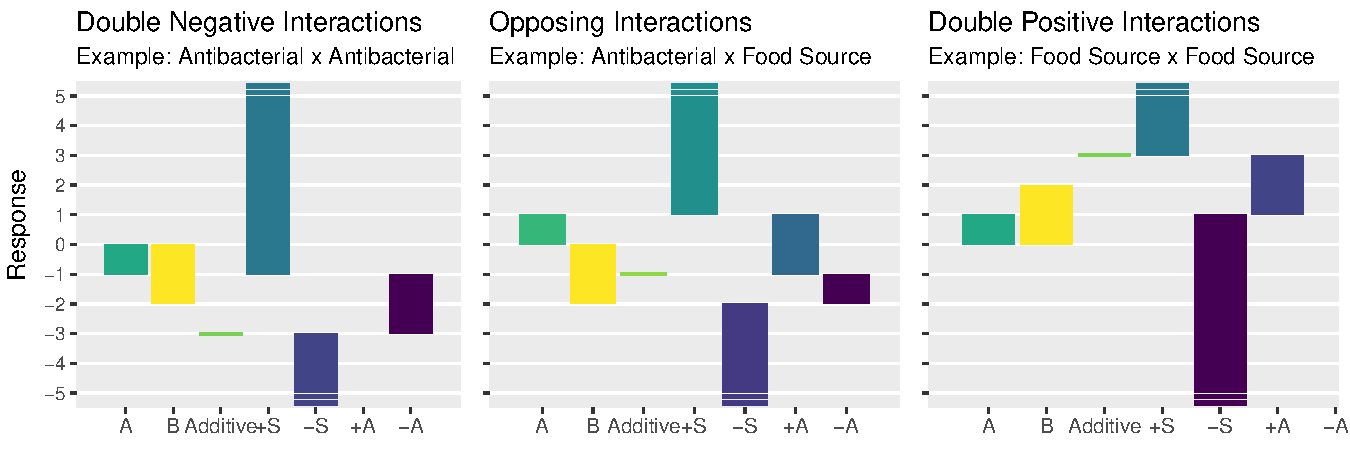
\includegraphics[width = \textwidth]{Scripts/Results/Plot_Interactions_Illustrative.pdf}
    \caption{Plots to illustrate the ranges of Piggott, Mattheai \& Townsend's reconceptualised interaction definitions \cite{Piggott2015}. Interaction definitions for three possible combinations of stressors with a negative or positive effect on organism fitness (A \& B) are depicted visually: i) Additive, the null hypothesis, ii) and iii), a positive or negative effect larger in absolute terms than the null hypothesis, and iv) and v), a positive or negative effect smaller in absolute terms than the null hypothesis.  A gradient effect indicates a definition range that continues towards $-\infty$ or $+\infty$, while the range of additivism is technically bounded by statistical significance rather than pure numerical distance. A positive antagonism is not possible for double negative interactions, while a negative antagonism is not possible for double positive interactions.}
    \label{fig:interaction_ranges}
\end{figure}

Eight nested multiple linear regressions were fitted to the data using a nested set of combinations of stressors. The simplest model (Complexity = 1) attempted to explain variation using only an intercept and the effects of eight individual stressors. The next simplest model (Complexity = 2) included the previous model's explanatory variables, but added all possible two-way stressor combinations as additional variables, and so forth, to the most complex model (Complexity = 8). This permitted us to determine statistically what level of interaction was predominant in the observed results. Linear regressions were compared using both a one-way ANOVA to F-test nested models, to apply an F-test to models, and Akaike Information Criteria test (AIC), to compare models with a penalty for number of estimated parameters \cite{Akaike1974}. 

A variation of the protocol used in Beppler \textit{et al.} \cite{Beppler2016} was applied to the data to detect 'emergent interactions', observed effects for an c-complexity stressor mixture that could not be predicted from the combined effects of their component ($c-1$)-complexity mixture observations. Predicted mean (eq. \ref{E:pred_mean}), standard deviation (eq. \ref{E:pred_sd}) and sample size (eq. \ref{E:pred_n} were calculated per isolate as follows: 
\begin{equation}
    m_c = \sum_{i = 1}^{c_n}\Big(\frac{m_c-1}{c_n}\Big)
\label{E:pred_mean}    
\end{equation}
\begin{equation}
    s^2_n = \sqrt{\sum_{i = 1}^{c_n}\bigg(\frac{(s^2_{n-1})^2}{c_n}\bigg)}
\label{E:pred_sd}    
\end{equation}
\begin{equation}
    n_c = \sum_{i = 1}^{c_n}\Big(\frac{n_c-1}{c_n}\Big)
\label{E:pred_n}    
\end{equation}

\mbox{where:}

\begin{small}
\setlength{\tabcolsep}{1pt}
\begin{tabular}{r p{11cm}}
    $c :$ & complexity of stressor mixture \\
    $c_n :$ & number of mixtures of $c$ complexity \\
    $m :$ & mean effect of mixture of complexity $c$ \\
    $n_c :$ & adjusted sample size of component--predicted effect of mixture of complexity $c$ \\
    $s^2_n :$ & adjusted summed standard deviation of component--predicted mixture of complexity $c$ \\
\end{tabular}
\end{small}

\section{Results}
\label{S:3}

\subsection{Rangefinding}
\label{S:3:1}

Isolates showed a variable response across the spread of rangefinding concentrations (\cref{fig:rangefinding}) with KUB5\_13, KUE4\_4, and the Nash's Field Soil Community generally proving the most able to grow regardless of stressor or concentration. The expected negative correlation between concentration and mean growth was not apparent. Azoxystrobin--exposed cultures did not appear to grow at any of the concentrations used.

\begin{figure}[H]
    \centering
    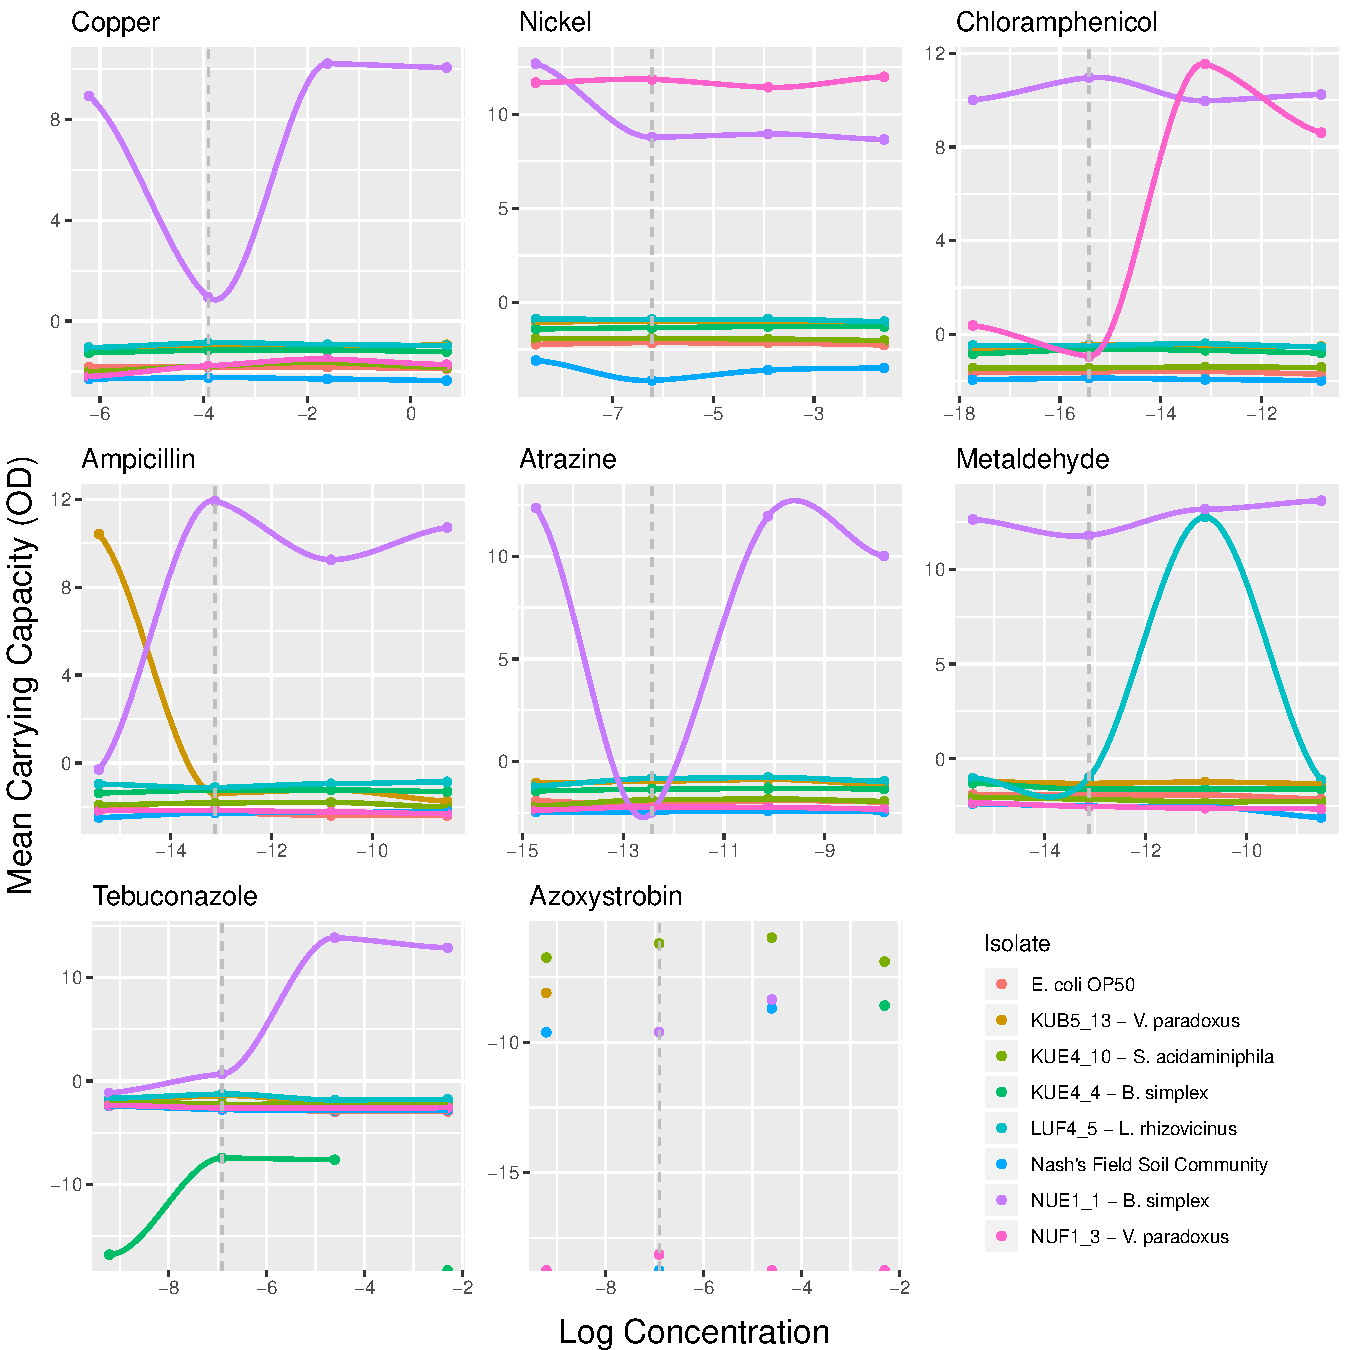
\includegraphics[width = \textwidth]{Scripts/Results/Bug_Rangefinding/plots_rangefinding.pdf}
    \caption{Maximum Optical Density at $\lambda$ = 590 nm over 48h growth, by isolate, across target concentration ÷ 10, target concentration (dotted grey line), target concentration × 10 and target concentration × 100 (see table \ref{tab:stressors}). Local area polynomial regression (LOESS) fitted to data points for illustrative purposes. n = 3 for all combinations of isolate, stressor and concentration. \textit{Note that Maximum OD was used to distinguish growth in the original rangefinding and thus is retained as a metric in this graphic.}}
    \label{fig:rangefinding}
\end{figure}

\subsection{Sample Sizes}
\label{S:3:2}

Due to a number of issues with isolate growth in liquid media and manual pipetting error of bacterial cultures, sample size varies across both treatments and isolates (\cref{tab:samples}). These small and variable sample sizes have affected the statistical significance of the data and analysis discussed below.

\begin{table}[ht]
\centering
\small
\begin{tabular}{l c c}
\toprule 
\textbf{Isolate} & \textbf{n Mean} & \textbf{n SD}  \\
\midrule
\rowcolor{gggrey}{LUF4\_5} & 3.4 & 1.7 \\
{KUB5\_13} & 2.8 & 1.8 \\
\rowcolor{gggrey}{NUF1\_3} & 2.8 & 1.8\\
{KUE4\_4} & 3.5 & 1.8\\
\rowcolor{gggrey}{NUE1\_1} & 2.6 & 1.6\\
{KUE4\_10} & 3.0 & 1.9 \\
\rowcolor{gggrey}{OP50} & 3.5 & 2.1 \\
{Soil Community} & 3.1 & 1.7\\
\bottomrule
\end{tabular}
\caption{Experimental issues caused sample sizes (n) to vary across isolates and stressor mixtures. This table gives mean sample size $\pm$ a standard deviation calculated on a per-isolate basis.}
\label{tab:samples}
\end{table}

\newpage
\subsection{Single Stressor Responses}
\label{S:3:3}

Isolates displayed a variety of responses (\cref{fig:sstress}) to the various stressors, growth in some cases apparently enhanced by the presence of most stressors (NUE1\_1, KUE4\_10, OP50, KUE4\_4, and the soil community) but in some cases diminished (NUF1\_3 and LUF4\_5) and in one largely unaffected (KUE4\_4). A bump in  the growth phase generally indicative of diauxic growth was strongly apparent in KUE4\_10, and sporadically present in the soil community, KUE4\_4, NUF1\_3 and NUE1\_1. 

\begin{figure}[H]
    \centering
    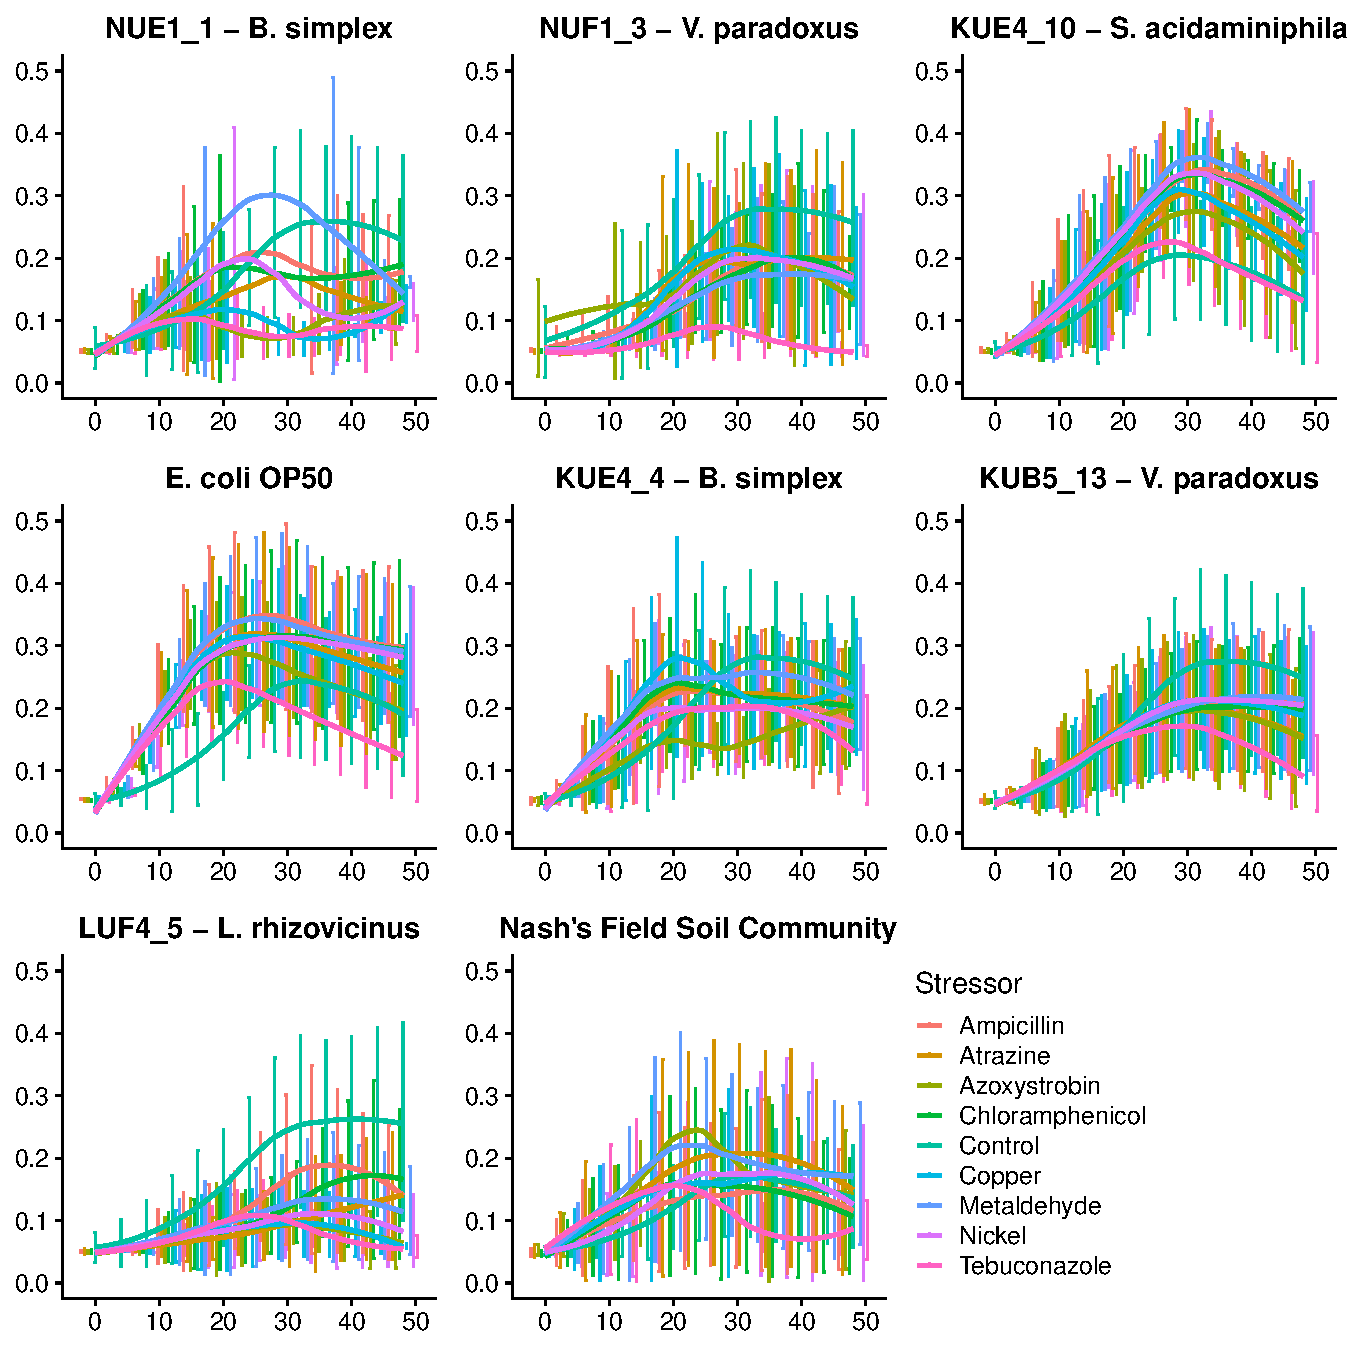
\includegraphics[width = \textwidth]{Scripts/Results/Final_Pipeline/single_stressor_plots.pdf}
    \caption{Effects of exposures of eight bacterial isolates to eight individual stressors, as well as a negative control on growth as measured by OD $\lambda$ = 590 nm, over 48 hours, with standard deviation. n = 1-4; see \cref{tab:samples}.}
    \label{fig:sstress}
\end{figure}

\newpage
\subsection{Growth by Stressor Complexity}
\label{S:3:4}

Modelling mean growth as either isolate or species versus mixture complexity did not reveal a statistically significant relationship (intercept = 0.03, $p = 0.07$) between complexity and growth. Isolate identity was a good predictor of variation except ($p < 0.05$), however, coefficient varied considerably in the case of one species, with \textit{B. simplex}'s KUE4\_4 displaying an intercept of -0.43 and NUE1\_1 an intercept of 0.63. 

\begin{figure}[H]
    \centering
    \includegraphics[width = \textwidth]{Scripts/Results/Final_Pipeline/growthXrichness.pdf}
    \caption{Mean Area under Growth Curve at $\lambda$ = 590 nm versus complexity of 256 mixtures of 1-8 chemical stressors. Individual data points, which represent a single mixture and isolate, are included as a measure of variance, and are displayed horizontally to reduce overlap.}
    \label{fig:growthXcomplex}
\end{figure}

\newpage
\subsection{Predicted Versus Observed Effect}
\label{S:3:5}

Patterns of observed versus predicted mean effect varied considerably among the species (\cref{fig:obsXpred}). Isolates KUB5\_13, NUF1\_3 and LUF4\_5’s have tight, linear distributions clustered around the 0 marks on both axes, while OP50, KUE4\_4 and the soil community’s observed effects fell largely below the predicted additive effect, especially at high levels of stressor complexity. KUE4\_10 and NUE1\_1’s patterns are more diffused across the additive line, but display a similar pattern of synergy at lower levels of complexity and antagonism at higher levels. This pattern is repeat across the majority of isolates, although LUF4\_5 shows a reversal of this pattern, and NUF1\_3 is clustered similarly but with greater x and y overlap between points of different richness.

\begin{figure}[H]
    \centering
    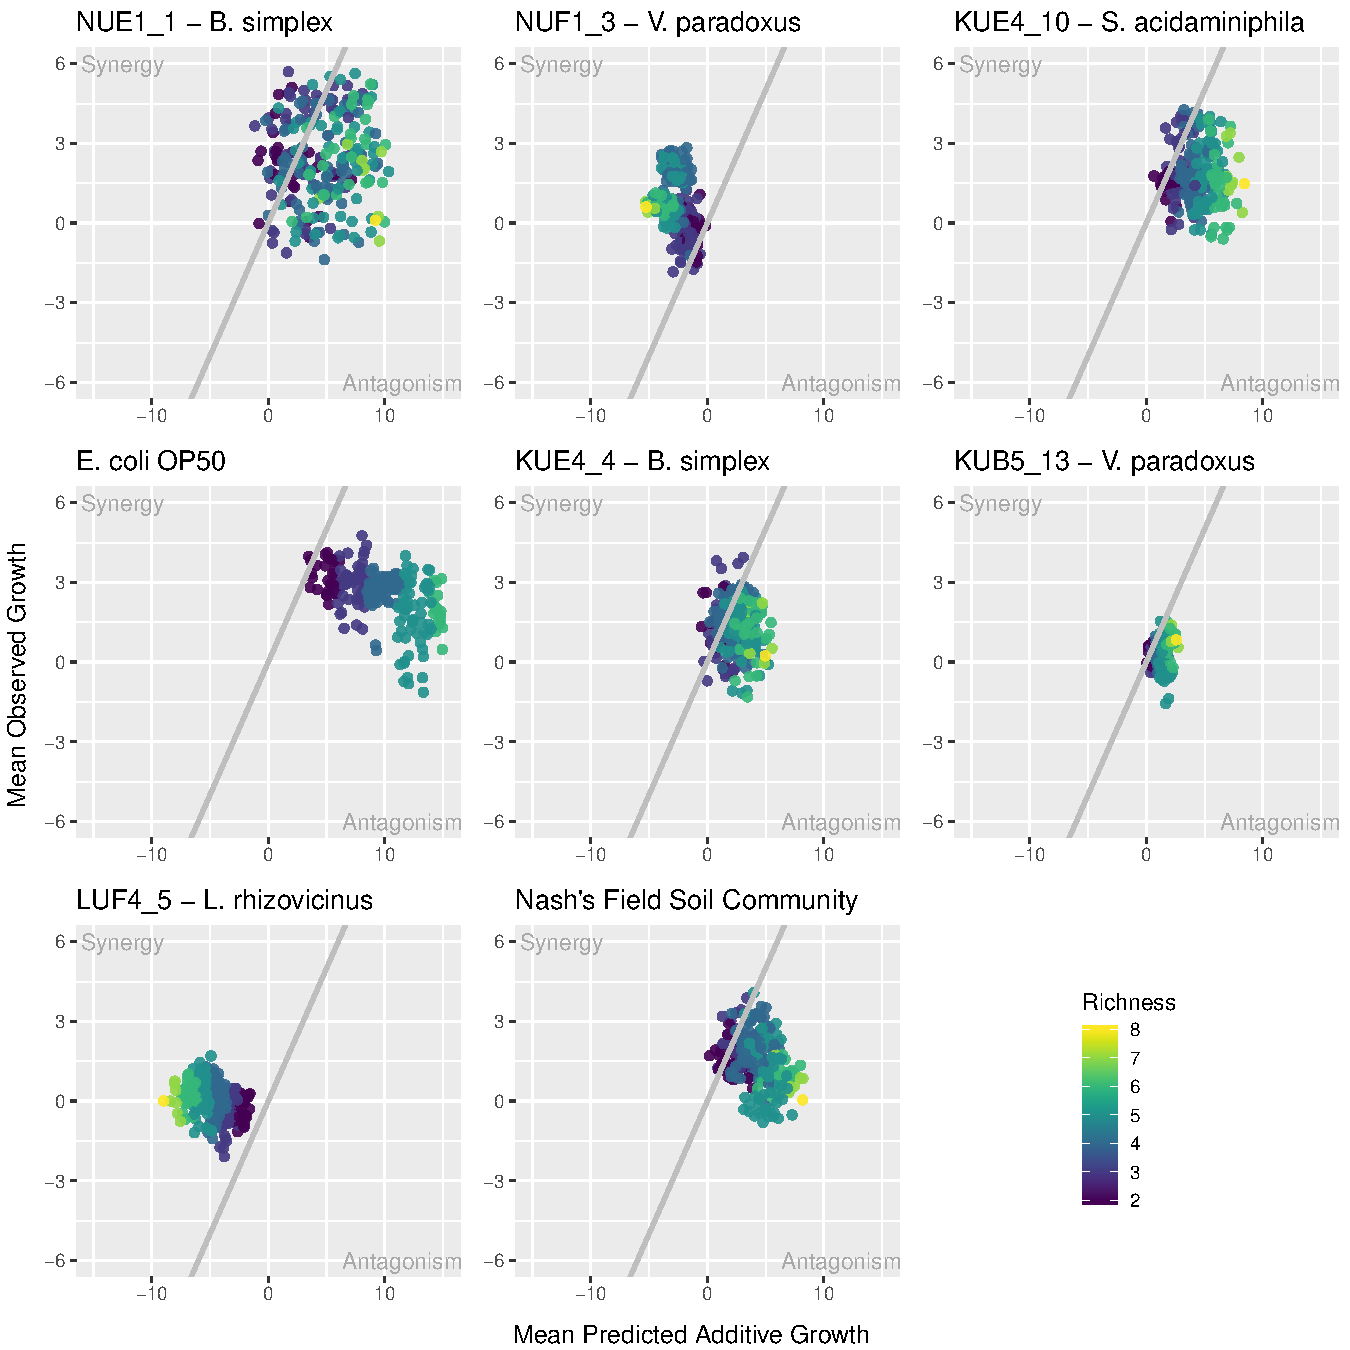
\includegraphics[width = \textwidth]{Scripts/Results/Final_Pipeline/ObservedXPredicted.pdf}
    \caption{Scatter plots of observed mixture stressor effect on mean area under growth curve (\ref{E:effect_calc}) compared to predicted mixture stressor effect on area under growth curve (\ref{E:pred_effect_calc}), colour coded by mixture complexity. Each point represents a single mixture of stressors. A grey line across the plot represents equality between predicted and observed result (accept the additive null hypothesis). Under basic definitions \cite{Bliss1939}, observed results higher than predicted are synergistic, and those lower results are antagonistic. \textit{Note that due to small sample sizes (\cref{tab:samples}), interactions that appear non-additive here may be rejected as not statistically significant in later graphics.}}
    \label{fig:obsXpred}
\end{figure}

\newpage
\subsection{Comparison of Linear Models of Higher-Order Mixtures}
\label{S:3:6}

A comparison of linear models of varying complexity (\cref{tab:lmodels}) showed F-values higher than the critical F-statistic (1.08 at $p = 0.05$) at $p < 0.05$ for the, 2-, 3- and 6-complexity models. Penalised for number of parameters, the 2-complexity model had a significantly lower AIC than other models. We can thus infer that a model of two-way interactions and single stressor effects best explains the variation seen in our data.

\begin{table}[H]
\centering
\tiny
\begin{tabular}{N N O P O N O O O N}
\toprule 
\textbf{Complexity} & \textbf{Number of Predictors} & \textbf{Residual Df} & \textbf{Residual Sum of Squares} & \textbf{Df} & \textbf{Sum of Squares} & \textbf{F-value} & \textbf{Pr(>F)} & \textbf{AIC Df} & \textbf{AIC Score} \\
\midrule
\rowcolor{gggrey}   1 & 8   & 6362 & 24990.99 & NA  & NA        & NA   & NA   & 10  & 26807.74 \\
                    2 & 36  & 6334 & 24310.99 & 28  & 679.99    & 6.41 & 0.00 & 38  & 26840.72 \\
\rowcolor{gggrey}   3 & 92  & 6278 & 24110.00 & 56  & 200.99    & 0.95 & 0.59 & 94  & 26894.15 \\
                    4 & 162 & 6208 & 23565.70 & 70  & 544.29    & 2.05 & 0.00 & 164 & 26909.64 \\
\rowcolor{gggrey}   5 & 218 & 6152 & 23441.87 & 56  & 123.83    & 0.58 & 0.99 & 220 & 26984.55 \\
                    6 & 246 & 6124 & 23210.18 & 28  & 231.68    & 2.19 & 0.00 & 248 & 26991.55 \\
\rowcolor{gggrey}   7 & 254 & 6116 & 23159.13 & 8   & 51.05     & 1.69 & 0.09 & 256 & 26991.97 \\
                    8 & 255 & 6115 & 23155.15 & 1   & 3.99      & 1.05 & 0.30 & 257 & 26992.38 \\     
\bottomrule
\end{tabular}
\caption{Comparison of the ANOVA and AIC parameters of eight nested multiple linear models of 1 to 8-way interactions, rounded to 2 decimal places. Calculated critical F-statistic of 1.04 at \textit{p} = 0.05.}
\label{tab:lmodels}
\end{table}

\newpage
\subsection{Interaction Type Prevalence}
\label{S:3:7}

The analysis of interaction type showed a relatively high incidence of T-test errors (133 in 1976; ~15\%), where the sample size of one of the compared populations was insufficiently large (n $<$ 3) to calculate a t-score. For most isolates additive effects prevailed (1744 in 1976; ~88\%), the exception being \textit{E. coli} OP50, where some non-additive effects were seen, especially at a complexity of 4 and above; negative antagonism accounted for slightly under half of the interactions observed (94 in 247; 38\%), while negative synergy was observed only at a complexity of 5 and in low quantities (5 in 247; 2\%).

\begin{figure}[hb]
    \centering
    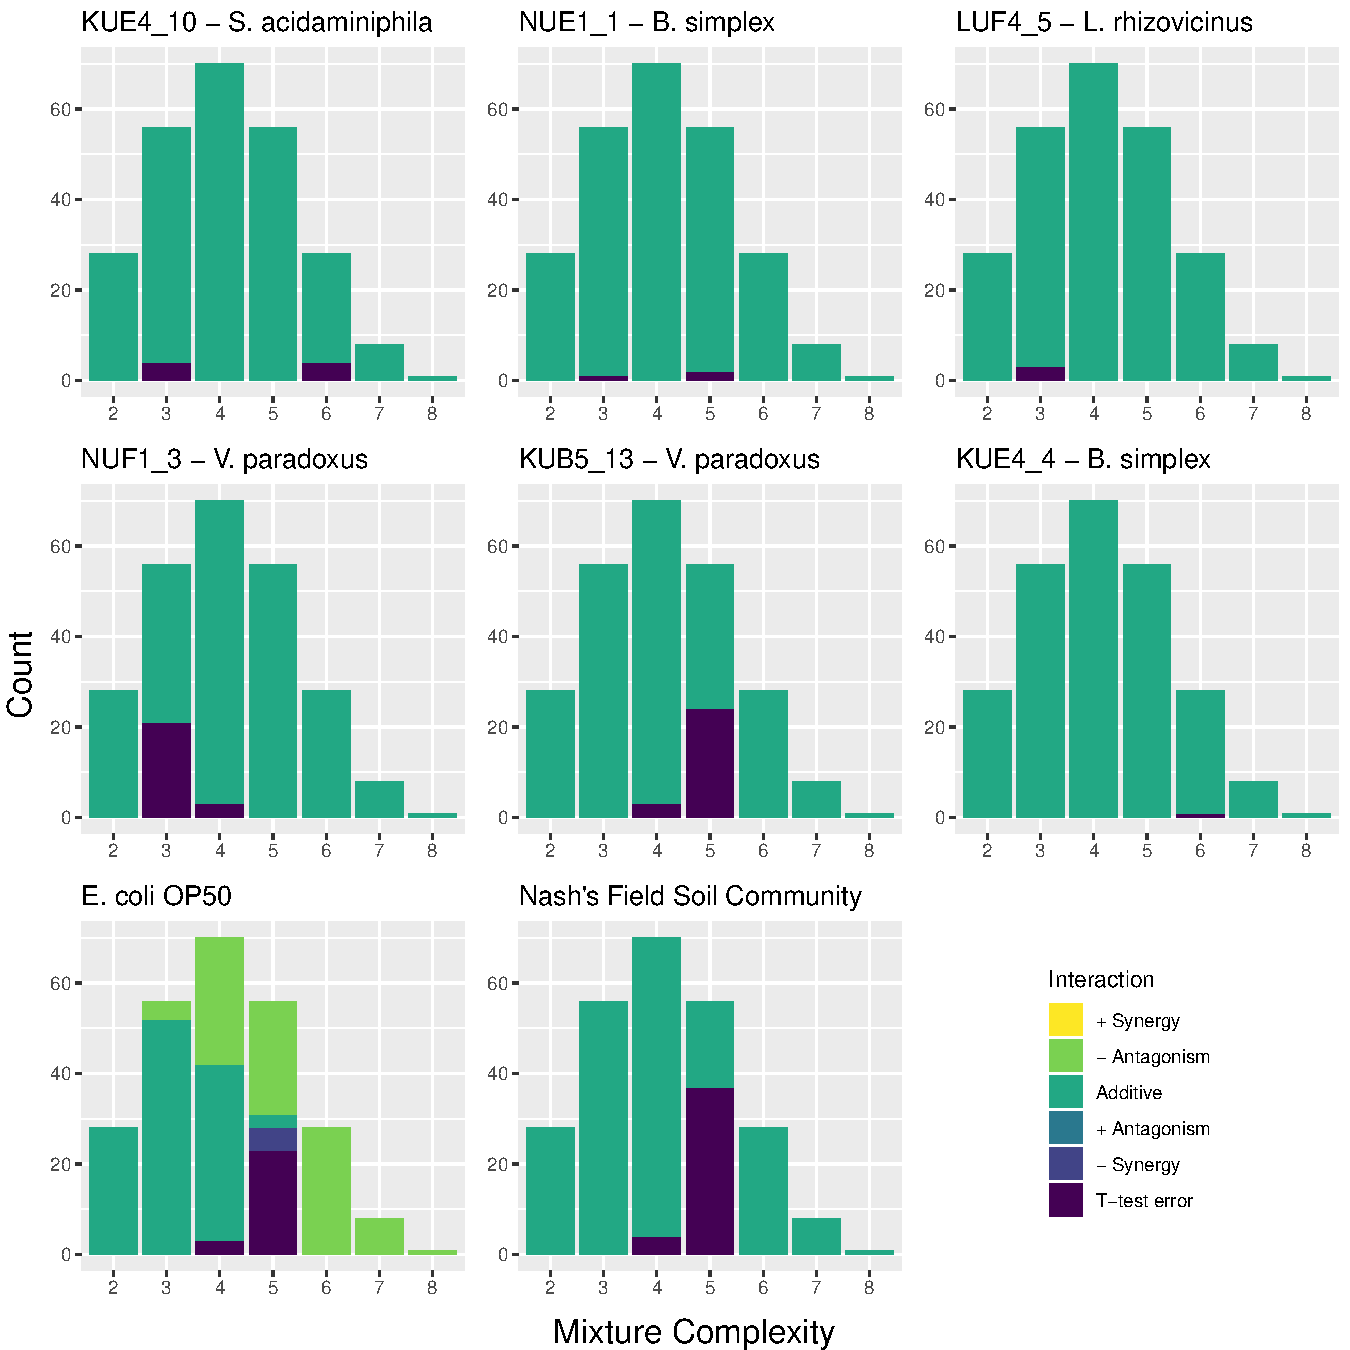
\includegraphics[width = \textwidth]{Scripts/Results/Final_Pipeline/histogram_interaction_basic.pdf}
    \caption{Count of observed interaction types, calculated by comparing observed stressor mixture effect to a predicted stressor effect of summed individual stressor effects (eq. \ref{E:pred_effect_calc}). Interaction direction and magnitude classified according to Piggott \cite{Piggott2015} (see \cref{fig:interaction_ranges}). All displayed interactions at $p < 0.05$, as determined by two-sample independent t-test. Sample size varies considerably between treatments and species (\cref{tab:samples}; cases where sample size was insufficient to calculate a t-score are marked `T-test error'.}
    \label{fig:histogram_interaction_basic}
\end{figure}

\newpage
\subsection{Emergent Interaction Type Prevalence}
\label{S:3:8}

Emergent interactions, effects of complex mixtures of stressors not predictable from their component mixtures at a level of complexity one lower were examined (eq. \ref{E:pred_mean}, \ref{E:pred_sd}, \ref{E:pred_n}) using two-sample independent t-testing. T-test errors represent a similar proportion of emergent effects observed (161 in 1752, ~9\%) . Non-emergent effects – “predicted” – dominate (1589 in 1752, ~91\%). Emergent synergy is non-existent, while two cases of emergent antagonism are present in NUE1\_1: a mixture of copper, nickel, metaldehyde and tebuconazole, and a mixture of copper, nickel, chloramphenicol, metaldehyde, tebuconazole, and azoxystrobin.

\begin{figure}[H]
    \centering
    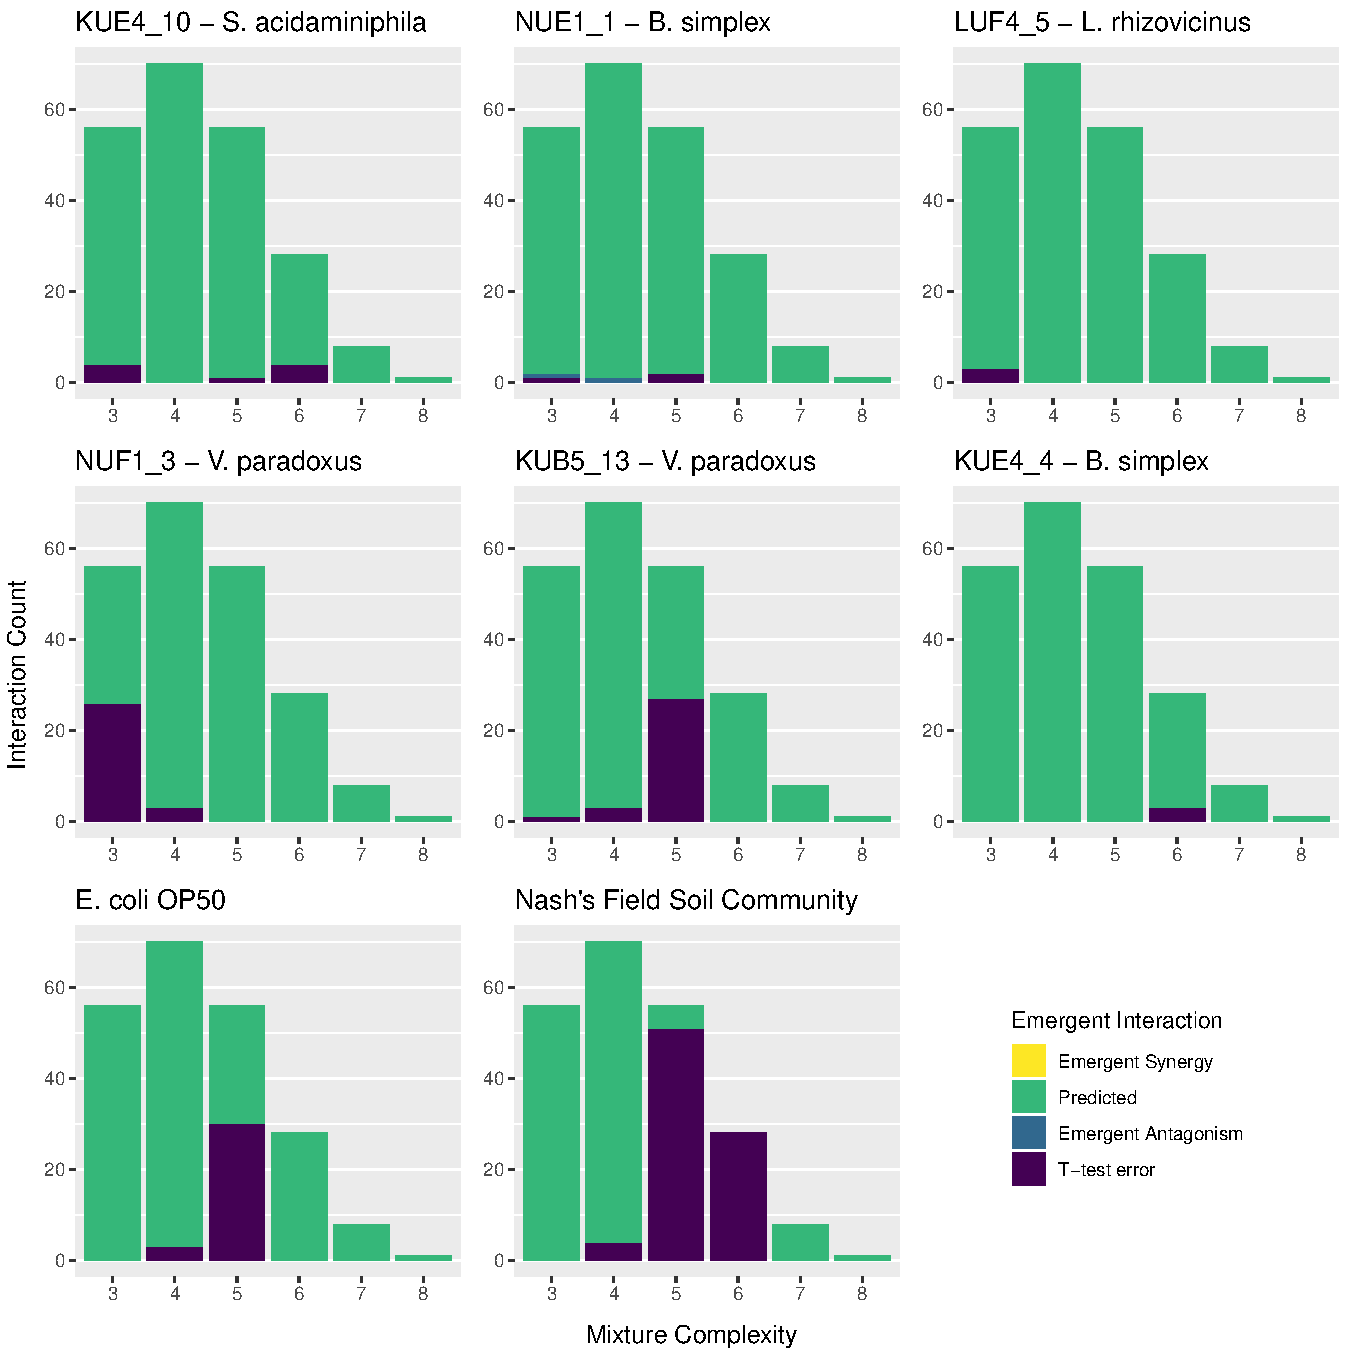
\includegraphics[width = \textwidth]{Scripts/Results/Final_Pipeline/histogram_interaction_emergent.pdf}
    \caption{Count of emergent interactions by complex mixture and isolate, as calculated by comparing observed mixture stressor effect (eq. \ref{E:pred_effect_calc}) to an additive prediction from component mixtures at a level of complexity one lower (eq. \ref{E:pred_mean}) using a two-sample independent t-test at $p < 0.05$. Sample size varies considerably between treatments and species (\cref{tab:samples}; cases where sample size was insufficient to calculate a t-score are marked 'T-test error'.}
    \label{fig:histogram_interaction_emergent}
\end{figure}

\newpage
\section{Discussion}
\label{S:4}

\subsection{Novel Findings}
\label{S:4:1}

The aims of this study were a) to determine if it was possible to predict the effects of complex mixtures of chemical stressors on a diverse range bacteria from their component single stressors and stressor mixtures, and b) to determine how prediction ability and mixture effects varied across isolates.

Although Figure 4 shows a relatively high incidence of observed effects deviating from the additive prediction, very few of these deviations are significant at $p < 0.05$ (Figure \ref{fig:histogram_interaction_basic}), the few cases of synergy and antagonism being limited to \textit{E. coli} OP50, where they were relatively common. A similar lack of emergent interactions (Figure \ref{fig:histogram_interaction_emergent}) was detected. 

However, a degree of inter-species variation at various levels of significance in response and interactive effect was present. The effects of individual stressors on growth varied considerably and frequently reversed between species, and different patterns of clustering between observed and predicted effects were observed in Figure 4. As discussed above, \textit{E. coli} OP50 showed the only significant non-additive interactions detected, although no similar pattern was observed at the emergent level. 

The study found interactive effects are limited to \textit{E. coli} and were not present in wild bacterial species. The strain used in this study, OP50, has a long history of use as a food source for \textit{C. elegans}. OP50 was likely selected as a feeder stock due to its rapid growth, and it is possible that mutations acquired over its recent history as a feeder species \cite{Tenaillon2016} have, in response to a lack of selection pressures unrelated to competition, led it to become both a faster grower in nutrient media and less tolerant to chemical stressors. Regardless, this finding does raise questions about the suitability of multiple stressor experiments that only consider effects of higher-order mixtures on lab-adapted model species, as their responses may not accurately reflect the response of more stress-tolerant wild species.  

At a regulatory and risk-assessment level, this study suggests that existing regulatory limits on common heavy metals, fungicides, insecticides and herbicides may be sufficient to protect bacteria from addition mixture effects, even at high levels of mixture complexity in the environment. More research is, however, required to determine how these mixtures affect communities over the long term, and in combination with other-non chemical stressors, such as temperature and land use change.  

\subsection{Caveats and Limitations}
\label{S:4:3}

A number of limitations apply to this study if overcome could affect the significance of detected interactions considerably.  Due to a combination of mistakes during the lab work phase of the study and the reticence of the strains KUB5\_13 and NUF1\_3 (\textit{V. paradoxus}) to grow directly in liquid media from cryogenic storage (perhaps unsurprising as the strains in question were sources from soil samples), the sample size in the case of a number of combinations (Table \ref{tab:samples}) was insufficiently large to detect non-additive effects at all but the highest p-values.  Greater replication of a smaller number of isolates would have permitted results to be declared with a greater degree of certainty. A further issue that may have affected OD readings for strains KUE4\_4 and NUE1\_1 (\textit{B. simplex}) is the tendency of \textit{Bacillus spp.} to aggregate within the well, creating considerable local variation in optical density. 

Additionally, due to the long preparation times for exposures, and experimental durations (96 hours from first the addition of media to plates to experiment end), well evaporation posed a non-random but difficult to account for influence on bacterial growth conditions, an additional stressor not part of the experimental design. Evaporation was most evident in peripheral wells (A1-–12, H1-–12, all X1 and X12 wells), and as stressor combination layout on the plates was not randomised between isolates or runs, it is probably that evaporation played a not-insignificant role in the observed effects of various treatments. Were a simpler level of treatment/isolate complexity used in simpler work, it would be possible to mitigate this effect by using only the inner wells of the 96 well plate, and by reduce experimental set-up time. 

Lastly, the incorporation of varying concentrations of stressors would have allowed the construction of dose response curves, calculation of inhibitory concentrations (ICs), and correspondingly the modelling of Bliss Independence \cite{Bliss1939} of stressors, which has been applied with some success to the issue of higher-order and emergent interactions in complex mixtures of antibiotics \cite{Beppler2016,Tekin2017a} 

\subsection{Next Steps}
\label{S:4:4}

A small but growing body of evidence conducted by researchers at the University of California has suggested that, in lab strains of \textit{E. coli}, the potential for higher-order interactions in complex mixtures of chemicals is far higher than previously assumed \cite{Beppler2016,Tekin2016,Tekin2017a}.  This study has undertaken a similar approach to a more diverse mixture of chemicals with mixed results; however, it is clear that existing attempts to understand the effects of the complex mixtures of stressors that define interactions in real-world ecosystems through simple interactions is insufficient.

With the increasing level of automation available in laboratories, it is crucial that further steps are taken to undertake work that will improve our understanding the role of complex stressor mixtures in contemporary ecosystems and study systems, and to develop effective strategies to protect and restore such effected ecosystems.

\section{Conclusions}
\label{S:5}

Recent advances in the understanding of higher-order effects of complex stressor mixtures suggest that effects are not as previous believed negligible. This study found predominantly additive effects at both the interaction and emergent interaction level; with non-additive effects largely limited to negative antagonism for \textit{E. coli} OP50 exposed to more complex mixtures. This suggests that studies that examine only lab species for interactions may not be fully applicable to wild populations, and thus that findings of significant higher-order mixture effects in lab species may not be a cause for concern about the ability of regulatory limits on chemical stressors to protect bacteria from mixture effects.

\section{Acknowledgements}
\label{S:6}
First and foremost I would like to thank my parents, without whose patience, support, and advice none of which would be possible.

Over the course of this project I benefited from the guiding influence of my official supervisors, Dr Tom Bell and Dr Emma Ransome, who were encouraging, supportive, educational, and, when necessary, firm. Dr Shorok Mombrikotb was also of indispensable assistance, providing isolates, soil samples, advice, and training on use of certain temperamental pieces of lab equipment. Chris, Nilita, Kate, Alice, and Meirion, also of Unit C, helped with other elements of my labwork.

In addition to the academic and commercial software and software packages cited in the main text and reference, I would like to thank to thank Chris West, who produced a batch Excel worksheet to .csv converter which was invaluable in the processing of my raw data. I've since learned that I had an R package that does the same thing installed the whole time...

This report was typeset in \LaTeX, using the online editor Overleaf, and the following packages: \textit{graphicx, amssymb, amsthm, rotating, booktabs, tabularx, array, siunitx,  textcomp, pdflscape, xcolor,  appendix, hyperref, final, threeparttable, scalefnt, inputenc, fontenc, amssymb, cleveref, float, geometry, amsmath}, which went some way to making \LaTeX a less frustrating piece of software to use.   

\section{References}
\label{S:7}
%% References
%%
%% Following citation commands can be used in the body text:
%% Usage of \cite is as follows:
%%   \cite{key}          ==>>  [#]
%%   \cite[chap. 2]{key} ==>>  [#, chap. 2]
%%   \citet{key}         ==>>  Author [#]
%% References with bibTeX database:
\bibliography{mendeley.bib}
%\end{thebibliography}
\begin{appendices}

\section{Data and Code}
\label{A:1}

All data, scripts, and calculations used in this study are available at: 

\url{https://github.com/samawelch/MScProject}

In addition to the packages cited in the main text, a variant t-test that took pre-calculated means, SDs and sample sizes as arguments was used as part of interaction classifications. This function was taken from an answer on Stack Overflow, and is cited here for want of a better place to do so \cite{Macro2012}.

\section{Nash's Field Treatments and Isolates}
\label{A:2}

The wild bacteria and soil communities used in this study were isolated from soil samples from the on-going Nash's Field herbivore exclusion experiment \cite{Allan2011ContrastingExperiment} at Silwood Park, Imperial College London, United Kingdom. Six isolates were selected from the 844 extracted by Dr Mombrikotb \cite{Mombrikotb2016}, with the intent of sourcing two control species, and two species that were present in both control and metaldehyde-treated plots. This, and the requirement that species be identified to a probability of 95\% limited species options to those selected. 

Dr Mombrikotb's and my notes on all species are available in the project Git repository in \verb|Data/Nash_Species| as the files \verb|Nash_Isolates_SBM.csv| and \verb|Nash_Isolates_SW.csv|.

\end{appendices}

\end{document}